\chapter{Experimentos e Resultados}\label{cap:experimentos}

Este capítulo apresenta a reconstrução integral dos escores da Fase 1 e a repetição da avaliação dos metamodelos. A comparação usa as mesmas tarefas, grupos e partições da referência histórica revisada; por isso, permite avaliar a mudança sem confundi-la com a alteração anterior de LOO por tarefa para validação por grupos. A avaliação continua retrospectiva sobre um acervo previamente explorado.

\section{Reconstrução Integral da Fase 1}

A auditoria dos dados brutos preservou 193 tarefas elegíveis, 179 nomes e 165 grupos. As oito exclusões por suporte insuficiente de classe permanecem documentadas. Não houve falha de carregamento ou mudança entre o alvo oficial da tarefa e o alvo padrão disponível no dataset. A identificação de grupos foi preservada, permitindo usar os mesmos folds externos na comparação.

Foram executados 57900 ajustes de classificadores, correspondentes a 193 tarefas, 60 pipelines e cinco folds estratificados por tarefa. Para todos os classificadores, inclusive SVM, foram usadas as mesmas linhas de treino e teste. A mediana numérica, o codificador categórico, os escalonadores e os seletores foram ajustados exclusivamente no treino de cada fold. O teste recebeu apenas as transformações já ajustadas. Transformações idênticas foram reutilizadas entre classificadores dentro do mesmo fold, sem compartilhar ajustes entre folds.

O processo registrou 0 falhas de ajuste, 0 escores agregados ausentes e 7703 avisos de convergência. Avisos de convergência são preservados como limitação do orçamento fixo, sobretudo do MLP com até 200 iterações; não são convertidos em convergência bem-sucedida. Um escore médio só é disponibilizado se os cinco folds foram avaliados. A matriz reconstruída possui 11580 posições de desempenho.

Nos pares tarefa/pipeline com escore observado nas duas versões, a variação média de acurácia balanceada dos classificadores da Fase 1, em pontos percentuais, foi: árvore de decisão: $-0{,}84$ p.p.; MLP: $-1{,}04$ p.p.; Random Forest: $-1{,}67$ p.p.; SVM: $-1{,}02$ p.p.; k-NN: $-1{,}65$ p.p.. Trata-se de uma média descritiva por par tarefa/pipeline, sem imputar os escores históricos ausentes ou atribuir peso igual aos grupos. Esses valores caracterizam a revisão da estimativa de desempenho dos classificadores; não devem ser confundidos com as métricas de ranqueamento dos metamodelos da Fase 2.

A validação dos artefatos verificou ausência de sobreposição entre treino e teste, cobertura de todas as linhas uma vez no teste e igualdade de amostras entre os 60 pipelines. Configuração, versões, hashes e índices de cada fold foram preservados em arquivos separados. Isso atende à reconstrução antes pendente; os escores históricos permanecem disponíveis para comparação, sem substituição silenciosa.

\section{Comparação Controlada das Condições}

Três condições foram avaliadas nas mesmas tarefas, grupos e partições externas: (i) escores e vetores históricos; (ii) escores reconstruídos com vetores históricos; e (iii) escores reconstruídos com vetores recalculados dos dados brutos. O segundo caso mantém a representação fixa para examinar o efeito dos novos alvos; o terceiro constitui a avaliação principal. As entradas das três condições usam precisão float32, como as matrizes históricas, preservando a mesma resolução numérica para tratar empates; os escores reconstruídos de origem permanecem em float64 nos artefatos da Fase 1. Em todos os casos, o ajuste de k e da padronização ocorre somente no treino interno.

A \autoref{tab:condicoesFaseUm} apresenta a comparação de Kendall ponderado. As médias de cada condição usam os grupos com métrica definida; a diferença é calculada de forma pareada, apenas com tarefas e grupos avaliáveis em ambas. Assim, a diferença pareada não precisa coincidir exatamente com a subtração de duas médias calculadas com suportes distintos. Os intervalos descritivos completos e as três condições estão nos CSVs.

\begin{table}[htbp]
\centering
\caption{Comparação da referência revisada com a reconstrução integral}
\label{tab:condicoesFaseUm}
\resizebox{\textwidth}{!}{\begin{tabular}{lrrr}
\toprule
Método & $\tau_w$ histórico & $\tau_w$ reconstruído & Diferença pareada \\
\midrule
Aleatório & $0{,}0024$ & $0{,}0012$ & $-0{,}0003$ \\
Média global & $0{,}3690$ & $0{,}4011$ & $0{,}0024$ \\
k-NN ajustado & $0{,}3995$ & $0{,}4280$ & $-0{,}0093$ \\
k-NN padronizado & $0{,}4138$ & $0{,}4539$ & $0{,}0090$ \\
Random Forest & $0{,}4309$ & $0{,}4768$ & $0{,}0059$ \\
\bottomrule
\end{tabular}}
\fonte{Autoria própria (2026).}
\end{table}

O k-NN apresentou $\tau_w=0{,}3995$ com escores históricos e $\tau_w=0{,}4280$ após reconstrução completa; Random Forest passou de $0{,}4309$ para $0{,}4768$. Esses resultados caracterizam a mudança no benchmark sob partições equivalentes. Não isolam causalmente apenas a imputação: também mudam a codificação por fold, a amostra da SVM, a semente explícita da PCA e, na condição principal, a recomputação dos vetores. A análise com vetor histórico fixo ajuda a distinguir o efeito dos escores daquele da representação. Os próprios rankings reais são recalculados e a cobertura pode mudar quando pipelines antes ausentes passam a ter escore; portanto, a diferença não isola ganho de capacidade preditiva sob uma única verdade de referência e um conjunto idêntico de itens avaliáveis.

Nos casos avaliáveis em ambas as versões, a mudança pareada de Kendall ponderado foi $-0{,}0093$ para k-NN, com intervalo descritivo $[-0{,}0282;0{,}0092]$ em 149 grupos, e $0{,}0059$ para Random Forest, com intervalo $[-0{,}0085;0{,}0202]$ em 151 grupos. O intervalo da mudança do k-NN ajustado abrange zero. O intervalo da mudança do Random Forest abrange zero. Assim, o aumento das médias gerais não deve ser interpretado isoladamente como melhoria da predição: também mudou o conjunto de casos com correlação definida.

O antigo valor de aproximadamente $0{,}5222$ para k-NN no LOO por tarefa não é a referência controlada desta seção. Ele usava outro protocolo e potencialmente mantinha tarefas relacionadas no treino; compará-lo diretamente aos resultados atuais atribuiria à Fase 1 diferenças de desenho da avaliação.

\section{Avaliação Principal dos Metamodelos}

A \autoref{tab:modelosRevisao} resume a avaliação dos metamodelos sobre a matriz reconstruída. O k-NN teve correlações definidas em 177 tarefas de 149 grupos. Os valores de k selecionados nos cinco treinos externos foram 5, 10, 10, 10, 10. Casos de correlação indefinida continuam contabilizados nos arquivos; NDCG e regret são preservados quando calculáveis.

\begin{table}[htbp]
\centering
\caption{Metamodelos sobre escores reconstruídos: médias por grupo}
\label{tab:modelosRevisao}
\resizebox{\textwidth}{!}{\begin{tabular}{lrrrrr}
\toprule
Método & Spearman & $\tau_w$ & NDCG@5 & Regret@1 & Tarefas/grupos ($\tau_w$) \\
\midrule
Aleatório & $-0{,}0114$ & $0{,}0012$ & $0{,}8843$ & $0{,}0785$ & 179/151 \\
Média global & $0{,}4277$ & $0{,}4011$ & $0{,}9522$ & $0{,}0260$ & 179/151 \\
k-NN ajustado & $0{,}4897$ & $0{,}4280$ & $0{,}9502$ & $0{,}0336$ & 177/149 \\
k-NN padronizado & $0{,}5148$ & $0{,}4539$ & $0{,}9533$ & $0{,}0259$ & 179/151 \\
Random Forest & $0{,}5293$ & $0{,}4768$ & $0{,}9632$ & $0{,}0207$ & 179/151 \\
\bottomrule
\end{tabular}}
\fonte{Autoria própria (2026).}
\end{table}

A diferença pareada Random Forest menos k-NN em Kendall ponderado foi $0{,}0515$, com intervalo descritivo de 95\% $[0{,}0255;0{,}0771]$. O intervalo descritivo sugere vantagem do Random Forest sobre o k-NN neste acervo. A conclusão é restrita ao acervo e ao protocolo; o Random Forest tem hiperparâmetros fixos e não houve comparação exaustiva de metamodelos. A \autoref{fig:modelosRevisao} mostra os intervalos das médias por grupo.

\begin{figure}[htbp]
\centering
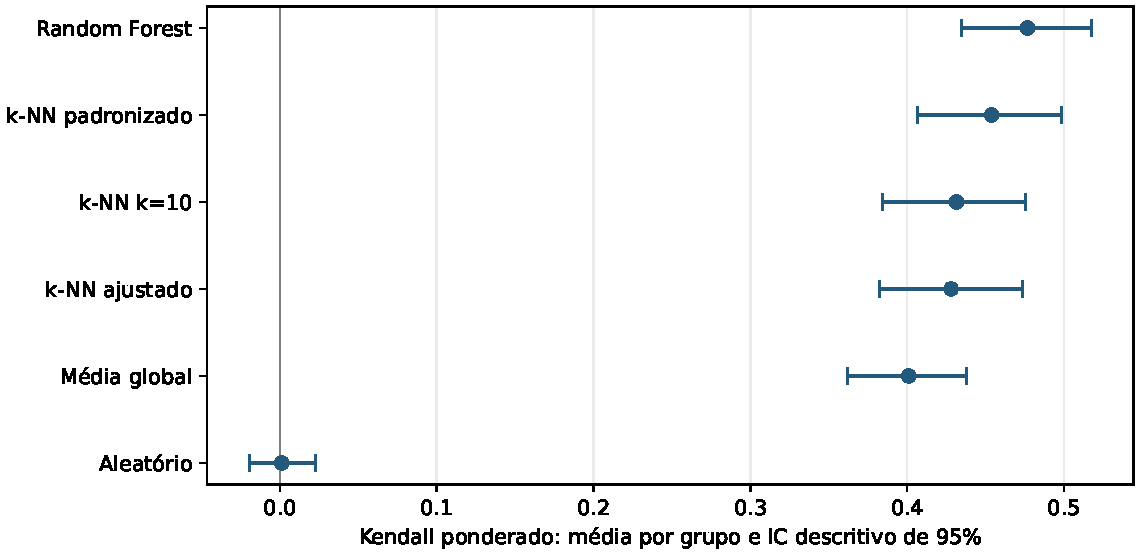
\includegraphics[width=.95\textwidth]{projeto/resultados/fase1_corrigida_2026/fase2/reconstrucao_completa/figuras/comparacao_modelos.pdf}
\caption{Kendall ponderado após reconstrução da Fase 1}
\label{fig:modelosRevisao}
\fonte{Autoria própria (2026).}
\end{figure}

O regret@1 foi $0{,}0336$ para k-NN, $0{,}0207$ para Random Forest e $0{,}0260$ para média global. A baseline aleatória apresentou NDCG@5 de $0{,}8843$. Isso reforça a necessidade de interpretar NDCG com as correlações e o regret: relevâncias próximas podem gerar NDCG alto sem recuperação exata do top-5. Kendall ponderado enfatiza inversões de maior peso, enquanto NDCG acumula relevância com desconto logarítmico.

\section{Diagnóstico de Falhas}

O k-NN ajustado apresentou 13 tarefas com Kendall ponderado não positivo e 16 com correlação indefinida. Foram registradas 14 tarefas com escores reais constantes e 2 com predição constante e escores reais variáveis. Uma correlação indefinida não é promovida a acerto nem convertida em zero. O diagnóstico liga cada task a tamanho, dimensionalidade, balanceamento, atributos constantes, distância ao vizinho de treino, predições e estado de avaliação. Entre as menores correlações definidas estão: tarefa 9976 ($\tau_w=-0{,}4184$, $N=2600$, $P=500$, proporção majoritária $0{,}5000$); tarefa 3512 ($\tau_w=-0{,}3760$, $N=600$, $P=60$, proporção majoritária $0{,}1667$); tarefa 363159 ($\tau_w=-0{,}3330$, $N=4531$, $P=1$, proporção majoritária $0{,}0603$). A inspeção permite reproduzir os casos, sem atribuir automaticamente suas falhas a uma característica isolada. Nenhuma das cinco associações exploratórias permaneceu abaixo de $q=0{,}05$ após ajuste Benjamini--Hochberg. Essas associações não demonstram causalidade nem explicam isoladamente a variabilidade.

\begin{figure}[htbp]
\centering
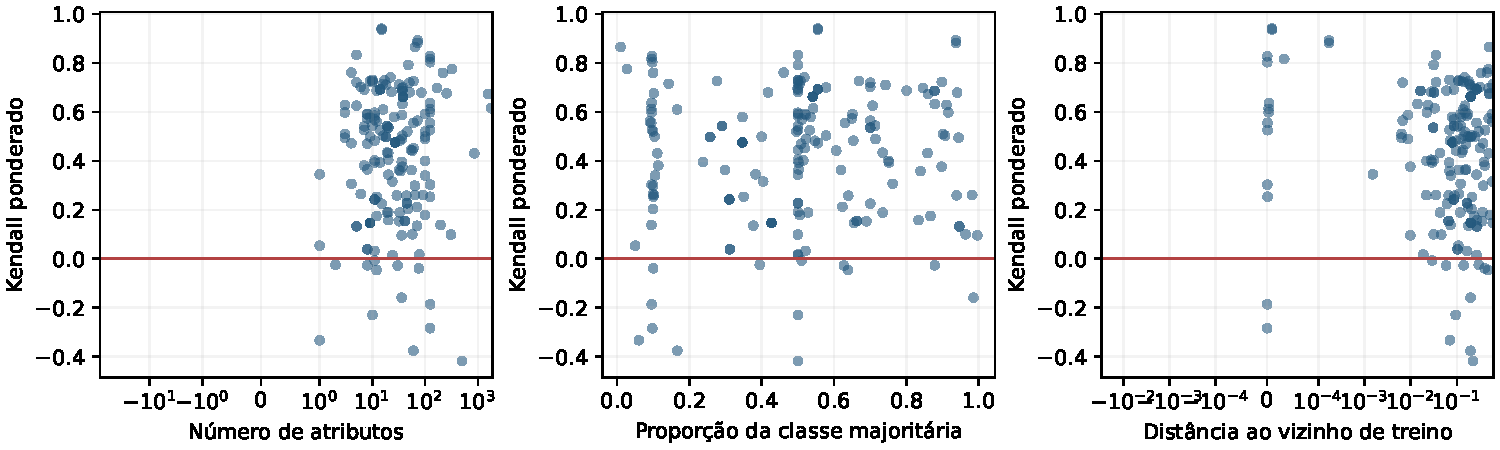
\includegraphics[width=\textwidth]{projeto/resultados/fase1_corrigida_2026/fase2/reconstrucao_completa/figuras/diagnostico_erros.pdf}
\caption{Diagnóstico do k-NN com escores reconstruídos}
\label{fig:errosRevisao}
\fonte{Autoria própria (2026).}
\end{figure}

\section{Discussão e Limitações}\label{sec:discussao}

A reconstrução corrige os dois problemas identificados na produção dos escores: estimar imputação antes da CV e usar amostra exclusiva da SVM. O controle também inclui codificação e seleção ajustadas no treino. A inclusão desses cuidados não implica aumento necessário das métricas; o objetivo é estimar desempenho sob condições comparáveis.

Permanecem como limites: avaliação retrospectiva, agrupamento conservador que pode não detectar todas as famílias, codificação ordinal de variáveis nominais, correlações de rótulos multiclasses dependentes de sua codificação e orçamento fixo de treinamento. A auditoria registra 30 tarefas somente categóricas e 18 com nomes sugestivos de identificadores ou caminhos. Esses indicadores exigem interpretação de escopo e não demonstram vazamento por si só; não foram usados para excluir tarefas após observar resultados. A representação descreve um conjunto rotulado completo e não cobre consulta sem rótulos. Intervalos de bootstrap dos grupos são descritivos, pois treinos de folds se sobrepõem. A comparação de metamodelos com o mesmo vetor não substitui uma ablação de representações.

O piloto anterior de 180 avaliações de hiperparâmetros permanece como evidência exploratória separada. O arsenal principal foi mantido em 60 candidatos para comparar protocolos e metamodelos sob espaço controlado. Expandir todo o arsenal, otimizar os metamodelos e avaliar conjuntos externos coletados após o desenvolvimento são próximos passos, sem tratar resultados de outros benchmarks como comparações numéricas equivalentes \cite{Gijsbers2024,Baratchi2024}.
